\documentclass[crop, tikz]{standalone}

\usepackage{tikz}
\usepackage{amsmath}
\usepackage{amssymb}
\usepackage[mode=buildnew]{standalone}

\usepackage{xcolor}


\usetikzlibrary{fit}

\definecolor{mred}{RGB}{214,39,40}
\definecolor{mgreen}{RGB}{44,160,44}


\begin{document}
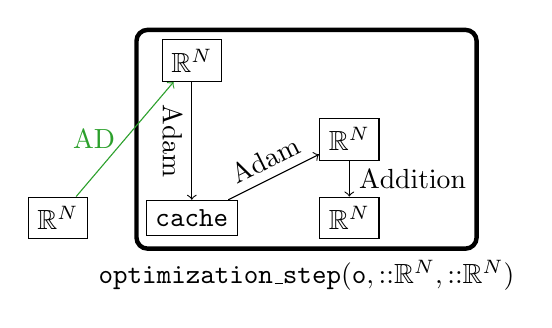
\begin{tikzpicture}
    \node[rectangle, draw] (R1)    at (.3,0) {$\mathbb{R}^N$};
    \node[rectangle, draw] (R2)  at (2, 2) {$\mathbb{R}^N$};
    \node[rectangle, draw] (cache) at (2, 0) {$\mathtt{cache}$};
    \node[rectangle, draw] (R3) at (4, 1) {$\mathbb{R}^N$};
    \node[rectangle, draw] (R4)	at (4, 0) {$\mathbb{R}^N$};
    \coordinate[right of=R3, xshift=.5cm] (addition);
    \node[fit=(R2)(cache)(R3)(R4)(addition),draw, ultra thick, rounded corners, label=below:$\mathtt{optimization\_step(o, ::}\mathbb{R}^N\mathtt{,::}\mathbb{R}^N\mathtt{)}$] (optimization_step) {};

    \draw[->] (R2) -- (cache) node[pos=.5, sloped, below] {Adam};
    \draw[->] (cache) -- (R3) node[pos=.5, sloped, above] {Adam};
    \draw[->] (R3) -- (R4) node[pos=.5, right] {Addition};
    \draw[->, mgreen] (R1) -- (R2) node[pos=.5, left] {\color{mgreen}AD};
\end{tikzpicture}
\end{document}